\documentclass[12pt,a4paper]{article}
\usepackage{rmpackages}																% usual packages
\usepackage{rmtemplate}																% graphic charter
\usepackage{rmexocptce}																% for DS with cptce eval
\usepackage{pdfpages}


%\cfoot{} 													% if no page number is needed
\renewcommand\arraystretch{1.5}		% stretch table line height

\begin{document}

\begin{header}
Chapitre 4 -- Le noyau de l'atome
\end{header}


\section{Le modèle de l'atome au collège}

\begin{figure}[h]
\center
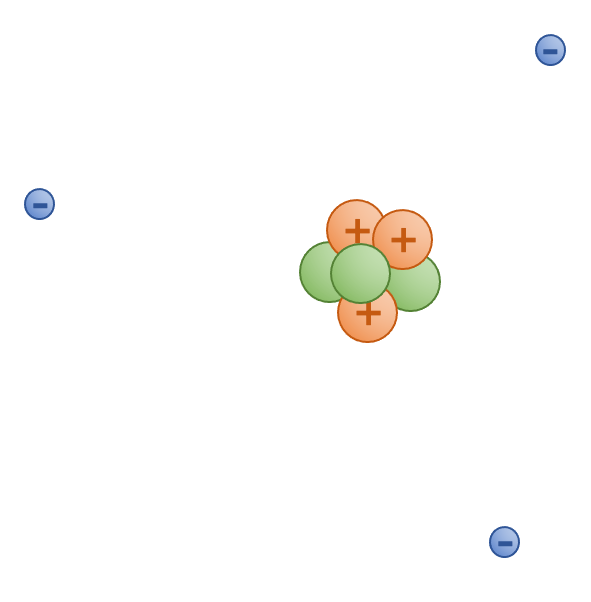
\includegraphics[scale=0.85]{images/atome.png}
\end{figure}

Les constituants du noyau sont les nucléons (protons et neutrons).

L'atome est neutre :
\begin{itemize}
\item[•] il y a autant de charges positives que de charges négatives ;
\item[•] il y a autant de protons que d'électrons.
\end{itemize}

\section{Écriture conventionnelle}

\begin{definition}
Pour représenter le noyau d'un atome de symbole X, on utilise la notation
{\Huge \bf
\[
^\text{A} _\text{Z} \text{X}
\]
}
\begin{itemize}
\item[•] \textbf{Z} est le nombre de \underline{protons}, aussi appelé \underline{numéro atomique} ;
\item[•] \textbf{A} est le nombre de \underline{nucléons }, aussi appelé \underline{nombre de masse}.
\end{itemize}
\end{definition}

\begin{itemize}
\item[•] \emph{L'atome représenté ci-dessus est le lithium et son symbole est Li.
Représente le noyau de cet atome en utilisant l'écriture conventionnelle.}

\[
^\text{6}_\text{3}\text{Li}
\]
\end{itemize}

\section{Quelle est la taille d'un atome ?}

\begin{definition}
Ordres de grandeur
\begin{itemize}
\item[•] Un atome mesure environ $\unit{10^{-10}}{m}$.
\item[•] Son noyau mesure environ $\unit{10^{-15}}{m}$.
\end{itemize}
\end{definition}

\begin{figure}[h]
\center

\includegraphics[scale=0.03]{images/qr_how_small_atoms_are.png}
\caption{Et si chaque atome avait la taille d'une myrtille... Une vidéo pour essayer de se représenter la taille d'un atome : \href{https://tinyurl.com/yygmqyqs}{https://tinyurl.com/yygmqyqs}.}
\end{figure}

\begin{itemize}
\item[•] \emph{Combien de fois le noyau est-il plus petit que l'atome ?}

\[
\frac{\mathrm{taille\ de\ l'atome}}{\mathrm{taille\ du\ noyau}} = \frac{10^{-10}}{10^{-15}} = 10^5.
\]
L'atome est $10^5$ fois plus grand que son noyau.

\item[•] \emph{Le schéma du début du cours est-il à l'échelle ?}

Le schéma n'est pas à l'échelle.
Le noyau est en réalité beaucoup plus petit.

\end{itemize}

\section{Quelle est la masse d'un atome ?}

\begin{center}
\begin{tabular}{l|c|c|c}
\textbf{Nom de la particule} & Neutron & Proton & Électron \\
\hline
\textbf{Masse} & $m_\mathrm{n} = \unit{1{,}675\times 10^{-27}}{\kilo\gram}$  & $m_\mathrm{p} = \unit{1{,}673\times 10^{-27}}{\kilo\gram}$ & $m_\mathrm{e} = \unit{9{,}1\times 10^{-31}}{\kilo\gram}$
\end{tabular}

\end{center}

\begin{itemize}
\item[•] \emph{Que remarque-t-on en comparant la masse d'un proton avec celle d'un neutron ?}

\[
\frac{m_\mathrm{n}}{m_\mathrm{p}} \approx 1.
\]
Les nucléons ont environ la même masse.

\item[•] \emph{Que dire de la masse d'un électron par rapport à celle d'un nucléon ?}

\[
\frac{m_\mathrm{n}}{m_\mathrm{e}} \approx 2000.
\]
Un nucléon est environ 2000 plus lourd qu'un électron.

\item[•] \emph{En utilisant les valeurs les plus précises possible, comparer la masse de l'atome de lithium représenté au début du cours avec celle de son noyau.
Pourquoi le nombre de nucléons est-il également appelé nombre de masse ?}

\begin{align*}
m_\mathrm{atome} &= 3 \times m_\mathrm{n} + 3 \times m_\mathrm{p} + 3 \times m_\mathrm{e} \approx \unit{1{,}005\times10^{-26}}{kg} \\
m_\mathrm{noyau} &= 3 \times m_\mathrm{n} + 3 \times m_\mathrm{p} \approx \unit{1{,}004\times10^{-26}}{kg} \\
\end{align*}
\[
\frac{m_\mathrm{atome}}{m_\mathrm{noyau}} \approx 1.
\]
L'atome a environ la même masse que son noyau.
Le nombre de nucléons correspond au nombre de particules qui contribuent majoritairement à la masse de l'atome, car les électrons ont une masse négligeable.

\end{itemize}

\section{Des particules électriquement chargées}

La charge électrique est une propriété fondamentale des particules qui composent l'atome.
Elle se note $q$ et son unité est le coulomb (C).
\begin{center}
\begin{tabular}{l|c|c|c}
\textbf{Nom de la particule} & Neutron & Proton & Électron \\
\hline
\textbf{Charge électrique} 	& neutre 	& positive 	& négative \\
							& $q_\mathrm{n} = \unit{0}{C}$ & $q_\mathrm{p} = \unit{+1{,}60\times10^{-19}}{C}$ & $q_\mathrm{e} = \unit{-1{,}60\times10^{-19}}{C}$
\end{tabular}
\end{center}

\begin{itemize}
\item[•] \emph{Comparer la charge électrique de l'électron avec celle du proton.}

\[
\frac{q_\mathrm{p}}{q_\mathrm{e}} = -1
\]
La charge du proton est l'opposée de celle de l'électron.
\end{itemize}

La charge électrique $\unit{1{,}60\times10^{-19}}{C}$ est appelée charge électrique élémentaire et on la note $e$ :
\[
e = \unit{1{,}60\times10^{-19}}{C}.
\]
La charge électrique du proton est donc $q_\mathrm{p} = +e$ et celle de l'électron est $q_\mathrm{e} = -e$.

\begin{itemize}
\item[•] \emph{En prenant l'exemple de l'atome de lithium, expliquer pourquoi l'atome est neutre.}

\[
q_\mathrm{atome} = 3 \times q_\mathrm{n} + 3 \times q_\mathrm{p} + 3 \times q_\mathrm{e} = 3 \times 0 + 3 \times e + 3 \times (-e) = \unit{0}{C}. 
\]
L'atome de lithium possède une charge électrique de \unit{0}{C}, il est donc neutre.
\end{itemize}


\section{Formation d'ions monoatomiques}

Parfois un atome peut gagner ou perdre un ou plusieurs électrons pour former un ion.
C'est le cas du lithium qui perd facilement un électron.
\begin{itemize}
\item[•] \emph{Quelle est la charge électrique de cet ion ?}

\[
q_\mathrm{atome} = 3 \times q_\mathrm{n} + 3 \times q_\mathrm{p} + 2 \times q_\mathrm{e} = 3 \times 0 + 3 \times e + 3 \times (-e) = e = \unit{1{,}60\times10^{-19}}{C}.
\]

\item[•] \emph{S'agit-il d'un cation ou d'un anion ?}

La charge est positive, c'est donc un cation.

\item[•] \emph{Quelle est la formule chimique de cet ion ?}
\[
\text{Li}^\text{+}
\]

\end{itemize}

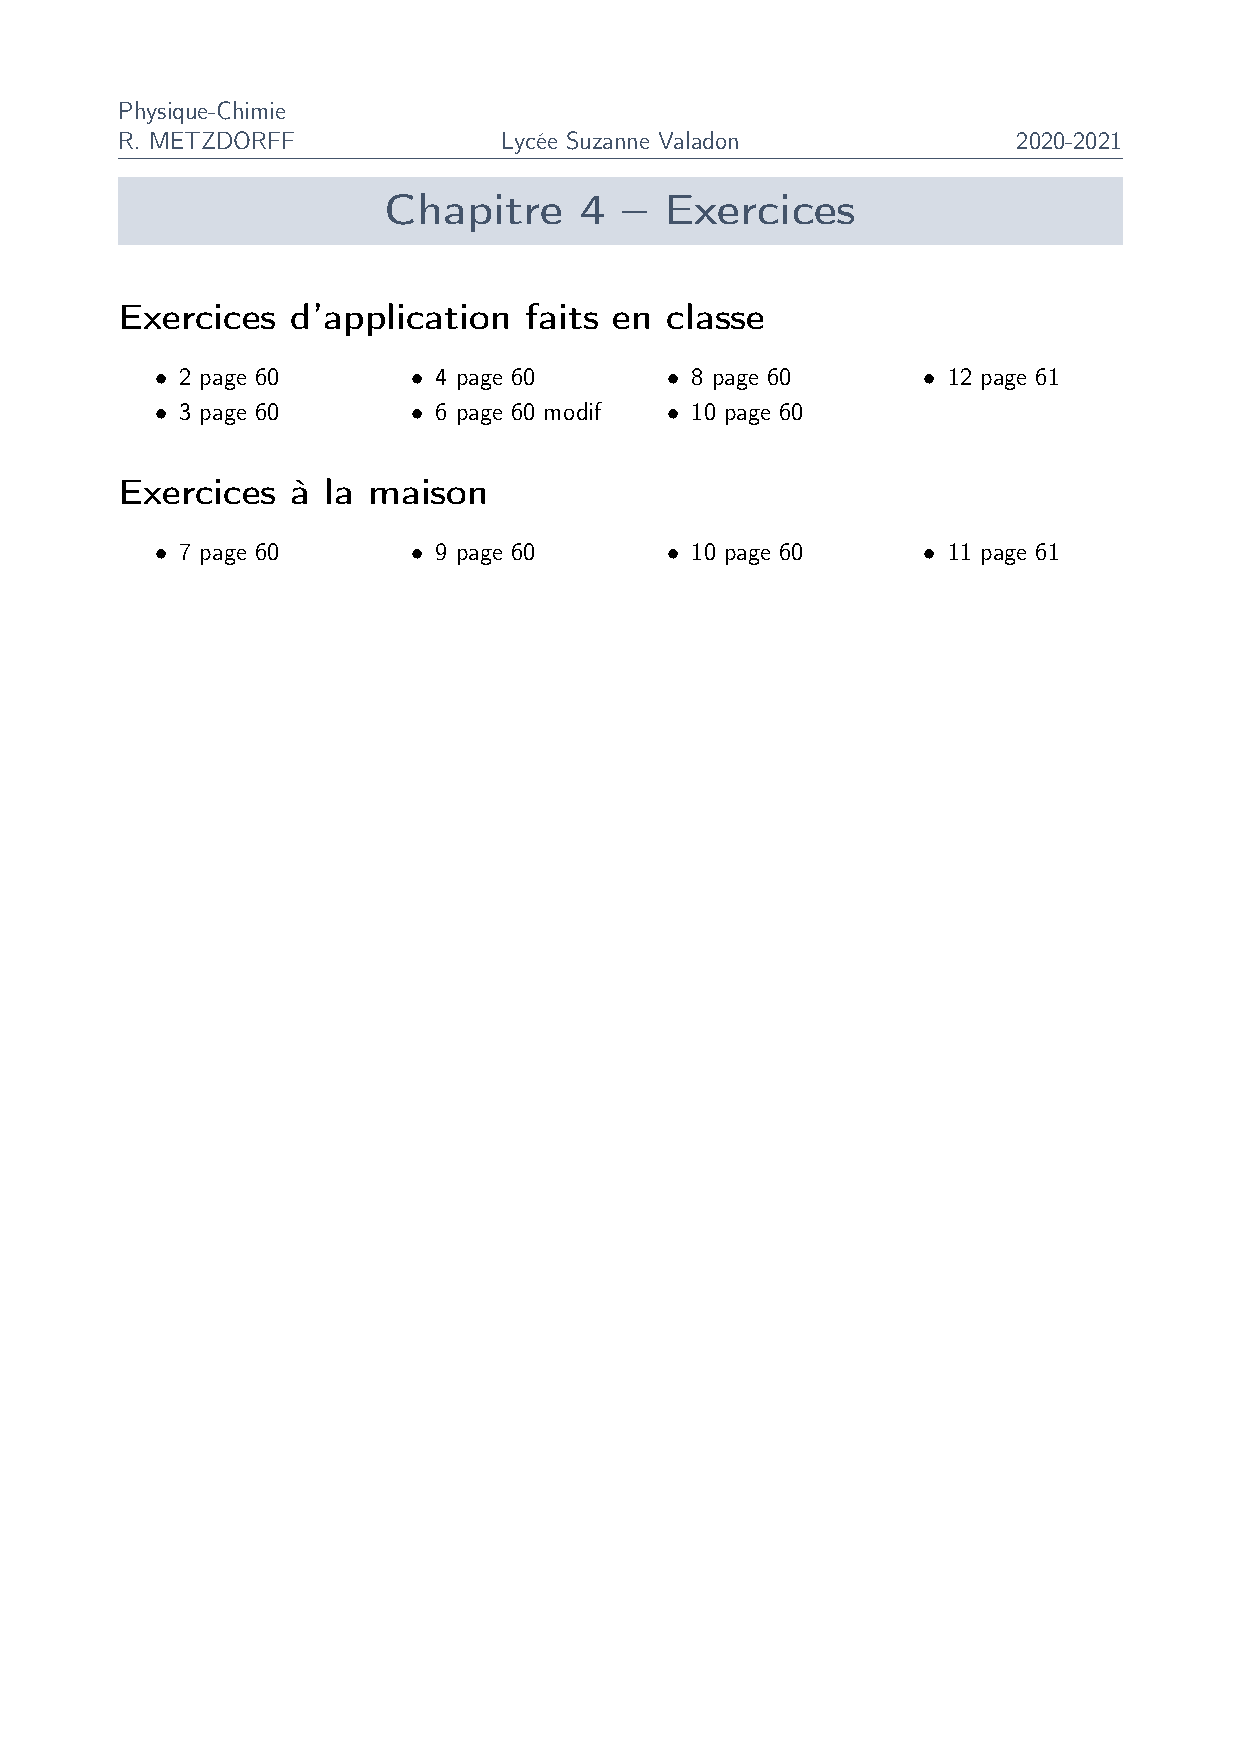
\includepdf[pages=-]{chap4_exos.pdf}


\end{document}